\documentclass[12pt]{article}

\usepackage[utf8]{inputenc}
\usepackage[T1]{fontenc}
\usepackage[french]{babel}
\usepackage{amsmath, amssymb}
\usepackage{stmaryrd}
\usepackage{fancyhdr}
\usepackage{comment}
\usepackage{hyperref}
\usepackage{graphicx}

\newcommand{\defeq}{\ensuremath{\; \hat{=} \;}}
\newcommand{\FOL}{\ensuremath{\textup{\tiny{}FOL}}}
\newcommand{\FOML}{\ensuremath{\textup{\tiny{}FOML}}}
\newcommand{\false}{\textup{ff}}
\newcommand{\true}{\textup{tt}}
\newcommand{\M}{\ensuremath{\mathcal{M}}}
\newcommand{\TLAp}{TLA$^+$}

\usepackage{xcolor}
\newcommand{\raph}[1]{\textcolor{red}{#1}}

\definecolor{myblue}{rgb}{0,0.5,0.8}
\newcommand{\mpar}[1]{\marginpar{\color{red}\footnotesize\raggedright#1}}
\newcommand{\bpar}[1]{\marginpar{\color{myblue}\footnotesize\raggedright#1}}
\addtolength{\marginparwidth}{1cm}
\long\def\stephan#1{{\color{myblue} #1}}
\newcommand{\TRUE}{\textsc{true}}
\newcommand{\FALSE}{\textsc{false}}

\newtheorem{prop}{Propriété}

\bibliographystyle{plain}
\pagestyle{fancy}
\setlength{\parskip}{12pt}

\title{%
  Compte rendu de stage de L3\\
  \vspace{8pt}
  \large On-the-fly Abstractions of Formulas in Proofs
Mixing First-Order Reasoning and Temporal Logic}
\author{Raphaël Le Bihan}



\begin{document}

\fancyhead[LEO]{Compte rendu de stage}
\fancyhead[REO]{Raphaël Le Bihan}
\fancyfoot[CEO]{\thepage}

\maketitle

Ce stage est effectué au Loria (Nancy), et a lieu du 08/06/2020 au 17/07/2020.
L'étudiant concerné est Raphaël Le Bihan en L3 au département d'informatique de l'ENS Paris-Saclay pendant l'année 2019-2020, l'encadrant du stage est Stephan Merz (Inria).
Le professeur supervisant le stage est Philippe Schnoebelen.

% METTRE TABLE DES MATIÈRES

\clearpage

\section{Introduction}

\subsection{Contexte}

TLA$^+$ est un langage de spécification utilisé pour la vérification de systèmes distribués \cite{lamport2002}.
% Il permet de décrire le comportement attendu d'un système par implémentations successives OSEF
Il permet de décrire le comportement attendu d'un système par des propriétés temporelles exprimées avec des formules logiques, et d'écrire des preuves formelles pour ces propriétés.
TLA$^+$ s'appuie sur la logique TLA (pour Temporal Logic of Actions), introduite en 1994 par Leslie Lamport \cite{lamport1994}.

TLA représente l'exécution d'un système comme une suite d'états, où un état est l'affectation d'une valeur aux différentes variables du système.
Elle doit donc permettre de construire des formules afin de raisonner temporellement sur ces états.
TLA est un cas particulier de logique modale du premier ordre (FOML pour First Order Modal Logic).
Elle est constituée de la logique du premier ordre à laquelle s'ajoutent deux opérateurs temporels : $\square$ indiquant qu'une propriété est toujours vérifiée, et $'$ un opérateur décrivant la valeur d'une expression lors de l'état suivant.
TLA autorise également la définition de nouveaux opérateurs $d(x_1, \cdots, x_n) \triangleq e$ où $e$ est une formule FOML.

TLA$^+$ est aujourd'hui distribué avec TLAPS \cite{TLAPSurl} (pour TLA$^+$ Proof System), un assistant de preuve permettant de vérifier la validité de propriétés exprimées avec TLA$^+$.
Pour vérifier une propriété avec TLAPS, un utilisateur doit écrire une preuve avec TLA$^+$, consistant en une suite d'étapes appelées obligations de preuve.
Chaque obligation de preuve contient une formule FOML à prouver, et les hypothèses à utiliser pour prouver cette formule.
Lors de la lecture de la preuve par TLAPS, chaque obligation de preuve est traitée par un prouveur automatique de logique classique du premier ordre (Isabelle, Zenon ou Z3) ou de logique temporelle (ls4).

\bpar{L'abstraction permet d'utiliser des outils qui ne comprennent qu'une partie des opérateurs sur des formules FOML.}
% Ces outils ne comprennent pas toute la FOML
Ces prouveurs automatiques utilisent des logiques ne comprenant qu'une partie de la FOML.
Par exemple l'opérateur $\square$ est défini en logique temporelle mais pas en logique du premier ordre.
Il est alors nécessaire de définir une méthode d'abstraction correcte de la FOML vers la logique du premier ordre (FOL pour First Order Logic) et la logique modale (ML pour Modal Logic). \raph{différence TL et ML}
Étant donnée une formule FOML $\phi$, on souhaite abstraire cette formule vers une formule FOL $\phi_\FOL$ telle que si $\vDash_\FOL \phi_\FOL$, alors $\vDash_\FOML \phi$ ; le principe est le même pour la logique modale.

Une méthode syntaxique appelée \og{}coalescing\fg{} (\og{}abstraction\fg{} en français) présentée en 2014 \cite{ARQNL2014} consiste à générer de nouveaux prédicats à partir des opérateurs FOML rencontrés n'étant pas reconnus dans la logique FOL ou ML.
On illustre cette méthode avec l'exemple suivant : l'opérateur $\square$ n'appartient pas à la logique FOL.
Etant donné un prédicat $P$ la formule FOML
\[ \phi = \square P \Rightarrow \square P \]
est valide.
On remarque qu'ici on peut déduire la validité de $\phi$ même sans savoir comment interpréter $\square$.
On abstrait alors la formule $\phi$ en :
\[ \phi_\FOL = \fbox{$\square P$} \Rightarrow \fbox{$\square P$} \]
où \fbox{$\square P$} est un nouveau prédicat.
$\phi_\FOL$ est valide et peut être prouvée en utilisant un prouveur automatique de logique du premier ordre.
On en déduit alors la validité de $\phi$ par correction de l'abstraction effectuée.

L'article de 2014 \cite{ARQNL2014} définit l'abstraction de la FOML vers la FOL et la ML et montre sa correction.
Il traite également le cas plus complexe de l'abstraction vers la FOL en présence d'opérateurs définis, et montre la complétude de l'abstraction pour la vérification de propriétés de sécurité et de vivacité, correspondant à la grande majorité des propriétés composants les spécifications en pratique. \raph{Utile de parler de la complétude ?}

\subsection{Objectifs du stage}

Afin de vérifier certaines obligations de preuve dans l'implémentation actuelle de TLAPS, il est parfois nécessaire de masquer explicitement des sous formules en les remplaçant par des opérateurs définis.
Sans cela la vérification de ces obligations de preuve échoue.
Pour illustrer ce phénomène on considère l'exemple suivant :
étant donnés une constante $z$ et un prédicat unaire $P$ dont l'interprétation peut varier au cours du temps (ceci sera introduit formellement dans la suite du compte rendu), on veut montrer que la formule
\[ \phi = (\forall x \; : \; \square P(x)) \Rightarrow \square P(z) \]
est valide.
On propose les deux preuves suivantes écrites avec TLA$^+$ et lues par TLAPS.
\begin{center}
  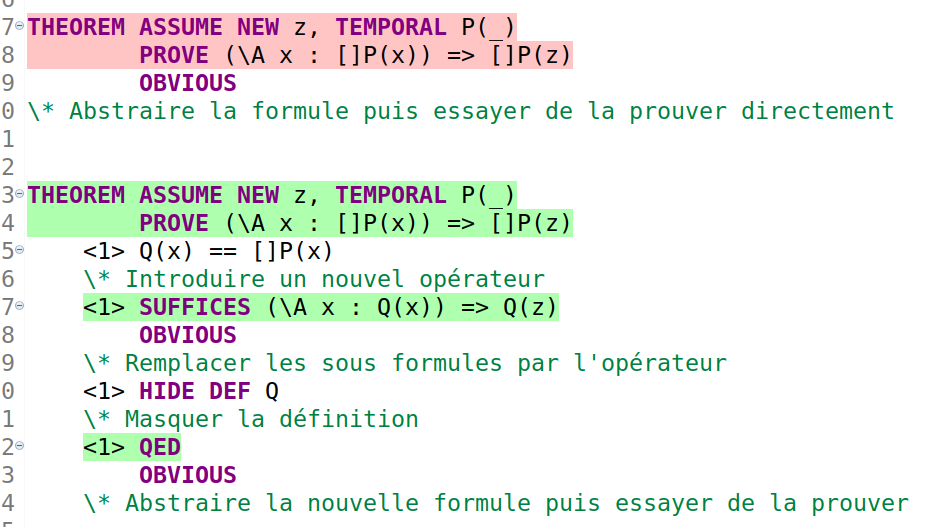
\includegraphics[width=0.8\linewidth]{tlaps_operateur}
\end{center}

La première preuve échoue car les sous formules $\square P(x)$ et $\square P(z)$ sont abstraits par des opérateurs différents, la formule FOL obtenue n'est donc plus valide.
La démarche utilisée dans la seconde preuve permet de vérifier la validité de $\phi$.

Un premier objectif sera d'étudier ce phénomène en confrontant ce résultat à la technique d'abstraction présentée l'article de 2014. On pourra chercher un moyen pour rendre possible de montrer $\phi$ sans avoir à introduire d'opérateur supplémentaire.


\section{Activités pendant le stage}

\subsection{Déroulement du stage}

Le stage a démarré le 08/06 et s'est terminé le 17/06, il a donc duré 6 semaines.
J'ai effectué pendant le stage les activités suivantes :
\begin{itemize}
\item
  Première semaine :
  j'ai lu l'article de 2014 sur le coalescing, lu et regardé des tutoriels et installé l'IDE pour travailler avec TLA$^+$ et TLAPS. J'ai fait quelques exercices pour m'entrainer à utiliser TLAPS ;
\item
  Deuxième semaine :
  j'ai fait quelques premiers tests avec TLAPS pour comprendre comment sont abstraites les formules dans l'implémentation actuelle.
  J'ai rédigé un fichier TLA$^+$ comparant les tautologies prouvables ou non en utilisant l'abstraction vers la FOL sans hypothèses supplémentaires.
  Le fichier contient également certaines idées pour modifier le processus d'abstraction afin de permettre de prouver plus de tautologies tout en conservant la correction.
  J'ai comparé les résultats du fichier avec les définitions données dans l'article.
\item
  Troisième et quatrième semaines :
  certaines tautologies ne sont pas prouvables une fois abstraites avec TLAPS, mais devraient l'être en utilisant les définitions dans l'article, il s'agit donc certainement d'une erreur d'implémentation.
  Plus généralement, il ne semble pas nécessaire d'après l'article d'utiliser des opérateurs pour masquer des sous formules comme présenté dans l'introduction.
  
  J'essaie de démontrer la propriété suivante : pour $\phi$ une formule FOML contenant des opérateurs définis, en notant $\widetilde{\phi}$ la même formule où on remplace les instances de l'opérateur par sa définition, si l'abstraction FOL de $\phi$ est une tautologie, alors l'abstraction FOL de $\widetilde{\phi}$ est également une tautologie.

  J'essaie pendant la troisième semaine de faire une preuve sémantique.
  Je veux montrer une propriété plus forte qui semble nécessaire pour utiliser l'hypotèse de récurrence.
  Je finis par trouver un contre-exemple à cette propriété.

  Je vois mal comment continuer, j'essaie pendant la quatrième semaine de faire une preuve syntaxique en utilisant la déduction naturelle.
  La plupart des cas de la récurrence sont triviaux sauf un.
  J'essaie d'utiliser un lemme, dont la preuve par récurrence est compliquée à cause de la définition de l'abstraction d'un opérateur défini posée dans l'article.
  Je propose une nouvelle définition, qui préserve la correction de l'abstraction.
\item
  Cinquième semaine :
  je commence la rédaction du compte rendu de stage.
\end{itemize}


\subsection{Définitions}

On présente ici les définitions utilisées dans la suite du compte rendu.

\subsubsection{Formules (ou expressions)}

\paragraph{Définition : formules FOML}
Etant donné un ensemble $\mathcal{O}$ d'opérateurs munis d'une arité, on définit une formule FOML récursivement
\[ e ::= \; x \; | \; v \; | \; op(\vec{e}) \; | \; e = e
  \; | \; e \Rightarrow e \; | \; \FALSE \; | \; \forall x : e \; | \; \nabla e \]
pour $op \in \mathcal{O}$, $x \in \mathcal{X}$, $v \in \mathcal{V}$ où $\mathcal{X}$ est l'ensemble des variables \emph{rigides}, $\mathcal{V}$ l'ensemble des variables \emph{flexibles}. $\mathcal{X}$ et $\mathcal{V}$ sont supposés infinis dénombrables et disjoints.
On n'autorise ici la quantification que sur les variables rigides.

On définit de même les 






\raph{%
TODO :
\begin{enumerate}
\item
  Confronter le CR et les documents de conseil des profs,
  \url{http://www.lsv.fr/~baelde/m1/reports.html}
  \url{http://www.lsv.fr/~leroux/To_be_downloaded/Teaching/Stages/conseils_informels_stage.pdf}
\item
  Rédiger + expliquer mes preuves
\item
  Envoyer le CR à Stephan + mes profs
\end{enumerate}
}

\bibliography{biblio_cr}

\end{document}